% Chapter Template

% popular unsolved research
%problem in the computer vision field


\chapter{Theoretical Background} % Main chapter title

\label{theory} % Change X to a consecutive number; for referencing this chapter elsewhere, use \ref{ChapterX}


\begin{itemize}
    \item How to choose the correct dataset?
    \item Which base architecture does learn human keypoints?
    \item How can Neural Networks understand image- and video data?
    \item How to optimize the inference of neural networks?

\end{itemize}

%\section{The Importance Of The Dataset}
%The quality of the data and the amount of useful information that it contains are key factors that determine how well a machine learning algorithm can learn
%https://learning.oreilly.com/library/view/python-machine-learning/9781787125933/ch04.html

\section{Architecture of Convolutional Neural Networks}
\glspl{CNN} help machines to understand image and video data.
The main building blocks of \glspl{CNN} are convolutional, pooling and fully connected layers.
\subsection{Types of convolutional layers}
The Convolutional Layers learn to detect specific features in the image data.
They do this with learned filters and activation functions presented in \autoref{activations}.
The learning process will be deeper discussed in \autoref{opt} and \autoref{cost}.
Via the stride $s$ and kernel size $k$ the feature maps can be reduced in size resulting in
learning coarser features.
Adding padding $p$ accordingly this decrease in size can be countervailed.
Given an input of size $I$ and filter of size $F$ the size of the output $O$ can be calculated as follows:

\begin{align}
    O_{conv}=\frac{I+2p-F}{s}+1
\end{align}

On the other hand, transposed convolution increases the size of the feature map.
It implements convolution with a modified input slice or convolutional filter, where this modification leads
to an increase of the feature map sizes~\cite{deconv}.
\glspl{DSC} combine depthwise and 1x1 pointwise convolutions, which can reduce the calculation efforts and increase
training and inference performance.
Having an input layer with three channels and a 3x3 kernel, the kernel is applied to each channel
separately depthwise on the input.
Now, the scalars on these three 3x3x1 filters are calculated and stacked together.
Afterwards, pointwise convolution is applied to each pixel of all channels.
The amount of times this 1x1 convolution is conducted on the input accounts for the number of output channels.
As an easy example, the kernel is presumed to be able to move 4x4 times across the image and expand the input to 256 output channels.
This would lead to the following calculation efforts for the original convolution
$256x3x3x3x4x4=110.592$.
When using the depthwise convolution for the three input channels the 3x3x1 kernel is moved 4x4 times
with $3x3x3x1x4x4=432$ calculations.
The pointwise convolution is applied 256 times according to the required output channels resulting in
$256x1x1x3x4x4=12.288$ calculations.
Summing up both calculations this gives $432+12.288=12.720$,
which means 11 times less calculations are needed for the depthwise convolution.
Replacing convolutional layers with \gls{DSC} can speed up performance~\cite{advanceddeeplearningpython}.
One network which intensively makes use of this trait, for example, is the MobileNet~\cite{mobilenet}.


\subsection{Pooling Layers}
Pooling layers can be used to increase the receptive field of deeper neurons and reduce the size of the filters
thus save calculation effort and speedup performance.
As for the convolution, the pooling operation is applied on the input in regard to $s$.
The size of each grid on which the pooling operation is calculated on the input slice is defined by the kernel $k$.
In contrast to the convolutional layers, no filters are learned.
The output size $O$ of the pooling operation can be calculated as follows:

\begin{equation}
    O_{pool}=\frac{I-F}{s}+1
\end{equation}

There are three very common pooling operations:
\begin{itemize}
    \item \textbf{Max pooling}: the maximum of each of the receptive fields is chosen.
    \item \textbf{Average pooling}: the average of each grid is calculated
    \item \textbf{Global Average Pooling (GAP)}: the average is calculated on the whole feature map with $I=F$
\end{itemize}
Pooling operations are usually combined with convolutions~\cite{advanceddeeplearningpython}.

\subsection{Fully Connected layers}
\gls{FC} connect all input pixels with each output.
In a convolutional network it can be used to refer the target labels from the learned features of the final convolutional
or pooling layers of the network.
Classification is one typical application for these layers, which will be further explained in \autoref{classification}.


\subsection{Non-Linearity Layer}
In the non-linearity layer an activation function $f$ performs an element-wise operation on the input feature map
$Y_i^l-1$ by creating the output activation map $Y_i^l$:

\begin{equation}
    Y_i^l=f(Y_i^l-1)
\end{equation}
with,
\begin{align}
    Y_i^l\in\mathbb{R}^{m_1^l\cdot m_2^l\cdot m_3^l} \\
    Y_i^l-1\in\mathbb{R}^{m_1^{l-1}\cdot m_2^{l-1}\cdot m_3^{l-1}} \\
    m_1^l = m_1^{l-1} \land m_2^l = m_2^{l-1} \land m_3^l = m_3^{l-1}
\end{align}
Where $m_1$ is the number of two dimensional feature maps or filters in convolutional layer $l-1$
with size $m_2 x m_3$.
As the calculus suggests, this layer is combined with a convolutional layer, where the filters ought to be
 learned~\cite{wikitumcnn}.
In the following commonly used activation functions for convolutional networks will be presented.

\subsubsection{Activation Functions}
\gls{ReLU} is a very popular activation function applied in the non-linearity layer.
With a threshhold at zero it is a piecewise linear function:

\begin{figure}
\centering
\caption{\gls{ReLU} activation function: $Y_i^l=max(0,Y_i^{l-1})$} \label{fig:ReLU}
\begin{tikzpicture}
  \draw[->] (-1, 0) -- (1, 0) node[right] {$x$};
  \draw[->] (0, -1) -- (0, 1) node[above] {$y$};
  \draw[scale=0.8, domain=-1.3:0, smooth, variable=\y, red] plot ({\y}, {0});
  \draw[scale=0.8, domain=0:1, smooth, variable=\y, red]  plot ({\y}, {\y});
  \draw[scale=0.8, domain=-1:0, dashed, variable=\y, blue] plot ({\y}, {0});
  \draw[scale=0.8, domain=0:0, dotted, variable=\y, blue] plot ({\y}, {\y});
  \draw[scale=0.8, domain=0:1.5, dashed, variable=\y, blue]  plot ({\y}, {1});
\end{tikzpicture}

\end{figure}
\[ f(x) =
  \begin{cases}
    x       & \quad \text{if } x \geq 0\\
    0  & \quad \text{if } x < 0
  \end{cases}
\]
\[ f'(x) =
  \begin{cases}
    1       & \quad \text{if } x > 0\\
    0  & \quad \text{if } x < 0
  \end{cases}
\]
Reasons for its popularity are first the efficient propagation of the gradient, which helps with vanishing gradients.
Second, since negative values become zero, the output volume is much more sparse, which provides robustness to
small changes and helps with noisy input data.
This is a great benifit for pictures, since many pixel values are not of high importance in reference to
the target label.
Third, the efficiency towards computation effort, thanks to the simple operations~\cite{wikitumcnn, advanceddeeplearningpython}.

However, one common problem is dying \glspl{ReLU}.
This happens when a weights' change is very high in $Y_i^{l-1}$ and in the next iteration $Y_i^l$ become very small
and thus stuck at the left side of \gls{ReLU}.
As a result learning stagnates and weights
stop adjusting properly in the backpropagation process.
Some modifications open up this strict threshold and help with this problem.

As examples can be named Leaky ReLU, \gls{PReLU}, \gls{ELU} and \gls{SELU} for easing up this threshold
below zero by making the function return values between
$[0;-\infty[$.

Since the presented experiments in \autoref{experiments} make use of the \gls{SELU} activation,
the next section further explains this function.


In 2017 Klambauer et Al. first introduced \glspl{SELU} in their research work of
\textit{Self-Normalizing Neural Networks} in which they successfully confront the named problem of dying
\gls{ReLU}~\cite{seluorigin}.
In comparison to the prior named activation function, \gls{SELU} additionally introduces normalization.
Each layer preserves the mean and variance from the previous layer, since positive and negative output values
are possible. These enable a shift process of the mean.
An extra parameter $\lambda$ scales values larger than zero.
The paper by Kambauer et Al. suggests to use a value slightly above one as 1.0507.
Due to the fact, that this parameter is larger than one, the gradient becomes larger than one as well, enabling
the activation function to increase the variance.
On the other hand a gradient very close to zero decreases variance.
Altogether, \glspl{SELU} confront the problem of vanishing gradients and in comparison to \glspl{ReLU} they do
not die.

Another activation function, which is usually used for the output layer of classification tasks in
convolutional networks is \textbf{softmax}.
\begin{equation}
    f(z_i)=\frac{exp(z_i)}{\sum_j=1^n exp(z_j)}
\end{equation}
Since this function outputs values between zero and one and the sum of $z$ is equal one $\sum_j=1^n exp(z_j)=1$
it will distribute the probabilities of the output neurons according to the amount of classes.
This means that this function will assign the probabilities to the given classes in a sequential order and help
to transfer the target labels.


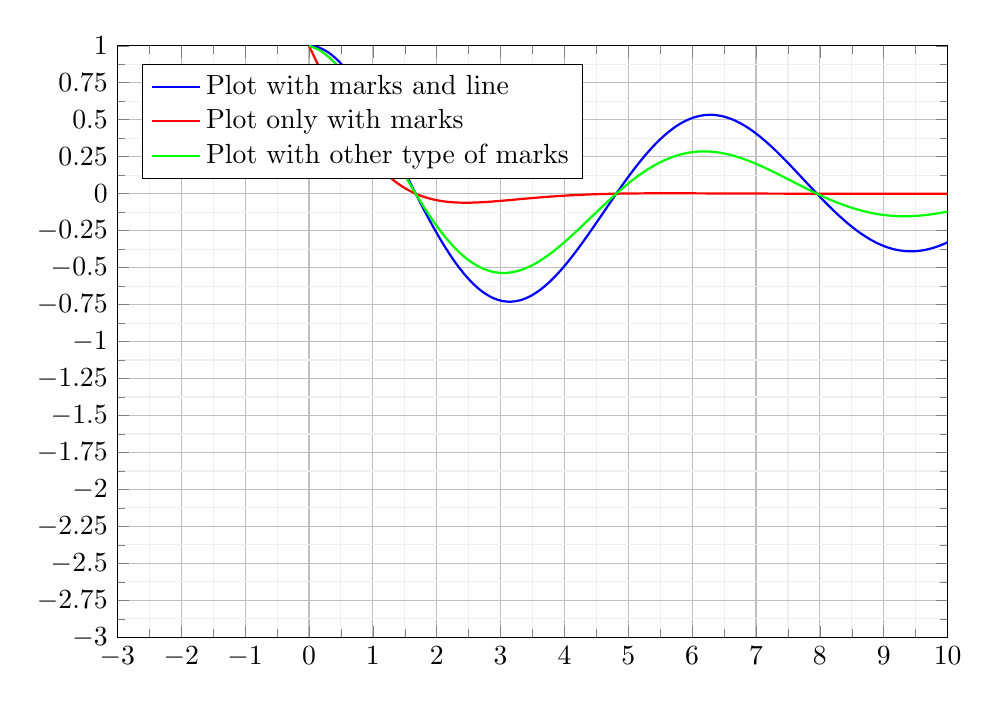
\begin{tikzpicture}
    \begin{axis}[
        xmin = -3, xmax = 10,
        ymin = -3, ymax = 1,
        xtick distance = 1,
        ytick distance = 0.25,
        grid = both,
        minor tick num = 1,
        major grid style = {lightgray},
        minor grid style = {lightgray!25},
        width = \textwidth,
        height = 0.75\textwidth,
        legend cell align = {left},
        legend pos = north west
    ]
        \addplot[
            domain = 0:30,
            samples = 200,
            smooth,
            thick,
            blue,
            ] {exp(-x/10)*( cos(deg(x)) + sin(deg(x))/10 )};
        \addplot[
            domain = 0:30,
            samples = 200,
            smooth,
            thick,
            red,
            ] {exp(-x)*( cos(deg(x)) + sin(deg(x))/10 )};
        \addplot[
            domain = 0:30,
            samples = 200,
            smooth,
            thick,
            green,
            ] {exp(-x/5)*( cos(deg(x)) + sin(deg(x))/10 )};
        \legend{
            Plot with marks and line,
            Plot only with marks,
            Plot with other type of marks}
    \end{axis}
\end{tikzpicture}

\subsection{Regularization}
Dropout and Batch normalization are commonly used regularization techniques for \glspl{CNN}.
With Dropout neurons are randomly dropped during training.
The amount of dopped neurons is specified via the dropout rate.
With this techniques the network is trained to not rely too much on the connected neurons.
In fact, every mini-batch training trains a different network architecture, since some neurons are excluded.

Batch normalization is applied to the hidden layers of a network.
It ensures that for every mini-batch the mean activation value
is close to zero and the standard deviation close to one.
With this it ensures that the activations will not explode or become to small.
Furthermore, overfitting is less likely to take place~\cite{advanceddeeplearningpython}.


\subsection{Optimization Algorithms}
\label{opt}
\begin{figure}[H]
    \centering
    \includegraphics[width=120mm, height=\textheight, keepaspectratio]{Figures/feature_maps_outpu.png}
    \decoRule
    \caption[HRNetV3: Prediceted Feature Maps]{HRNetV3: Predicted 9 feature map classes of the output layer of the
    human part detection module}
    \label{fig:feature-maps-output}
\end{figure}
Optimizing the weights of a neuronal network is a crucial step in the training life cycle of deep learning.
When the in \autoref{method} presented neural network has processed the input image and calculated several feature maps throughout the process,
at the end it predicts 9 feature maps of body parts for example for the head, arms, torso, and legs for the human parts
detection module~\ref{fig:feature-maps-output}.
With the help of a loss function, the error is then calculated for the predicted pixels in comparison to the truly labeled
pixels.
\subsubsection{Backpropagation Process}
The optimizer updates the network parameters $\theta \in \mathbb{R}^d$, which result in learned filters predicting several feature maps at
the different stages of the network.
The updates are performed accordingly to the calculated error from the loss function $\mathcal{J}(\theta)$ via the
so-called Backpropagation process, since the updates are passed backwards through the network.
This backward optimization process is performed by the calculations of the chosen optimizer.
The goal of the optimizer is to minimize the error.
There, it makes use of gradient descent to update the network's weights, biases and activation functions, in opposite direction
of the gradient.\\
Figuratively speaking, a weight could be imagined as a hill.
The updates then will follow the direction of the slope downhill until the valley is reached.
Whereas the valley represents a local minimum~\cite{optimizersoverview}.
\\\mbox{}\\
There are three variants for gradient descent:\\
\textbf{\gls{BGD}}, which calculates the gradients $\theta$ for the entire training dataset.
The problem here is, that most of the time this would not fit into the RAM.
For example, there were problems with data overflow when training was conducted with more than 12 images at a time, however, the image size was even reduced
to 320x240.
Another drawback is, that gradients for similar examples must be recalculated before each update, leading in redundant computations.\\
\textbf{\gls{SGD}} confronts this problem by performing updates for each training example input image $x_i$
and mask label $y_i$.
This optimization process is much faster.
Moreover, the updates are of more variance when random training examples are chosen.
A drawback however is, even if jumping around may result in finding another better local minimum, it may also
lead to constantly overshooting the exact minimum.
Against this problem, slowly decreasing the learning rate may help and lead to similar convergence as for BGD.\\
\textbf{Mini-Batch Gradient Descent} is the most common variant for gradient descent since it combines both the aspects of
\gls{BGD} and \gls{SGD}.
The updates are conducted for every mini-batch of \textit{n} training samples.
This reduces the variance of parameter updates and leads to less jumping around, which all in all results in more stable
convergence~\cite{optimizersoverview}.
\\\mbox{}\\
In the following section an overview of optimizers will be presented in reference to the used ones in ~\autoref{experiments}, which are
\gls{SGD}, \gls{Adam} and \gls{Nadam}.


%
\glsreset{SGD}
\subsubsection{\gls{SGD}}
\gls{SGD} is one of the first optimizers and still commonly in use.
Already in 1951, it was publicly reported by Robins and Sutton et Al~\cite{sgd}.
Now given the parameters of a neural network $\theta$, such as weights, biases and activation functions, here via an input image
$\mathfrak{x}$ and associate labels $\mathfrak{y}$ the Backpropagation process is defined under the gradient $\nabla$
from the calculated loss function $\mathcal{J}$.
The adaption of the parameters then is performed stepwise by the learning parameter $\eta$.


\begin{equation}
    \theta = \theta - \eta\cdot\nabla_\theta\mathcal{J}(\theta;x;y)
    \label{eqn:sgd}
\end{equation}

The \gls{SGD} optimizer updates a weight $\mathrm{w}$ in a way to reduce the loss function $\mathcal{J}(\mathrm{w})$ and find
the local minima of the parameters.
As already mentioned, this is one of the problems with pure \gls{SGD}, since it will very likely become stuck in a local minimum or
saddlepoint, where one slope goes up and the other one down.
Furthermore, it converges slower compared to newer optimizers~\cite{optimizersoverview, optimizersexplained}.
\\\mbox{}\\
\textbf{Momentum}, first proposed in 1999 by Qian et Al.~\cite{momentum}, can help to get faster to the local minimum.
This is accomplished by an additional term that is added to \gls{SGD}.
A constant fraction $\gamma$ is multiplied with the last parameter update $\mathfrak{v}_t$ to $\theta$.

%\begin{align}
%    \theta_t = \theta_t - \eta * \nabla\mathcal{J}(\theta_{t})+\gamma\mathfrak{v}_{t} \label{eqn:momentum:1}\\
%    \mathfrak{v}_t = \nabla\mathcal{J}(\theta_{t-1})+\mathfrak{v}_{t-1} \label{eqn:momentum:2}\\
%    \theta_t= \theta_t - \eta * \nabla\mathcal{J}(\theta_{t})+\gamma\sum_{\tau=1}^{t}\eta * \nabla\mathcal{J}(\theta_{\tau}) \label{eqn:momentum:3}
%\end{align}
\begin{align}
    \theta = \theta - \mathfrak{v}_t \label{eqn:momentum:1}\\
    \mathfrak{v}_t = \gamma\mathfrak{v}_{t-1} + \eta\cdot\nabla_\theta\mathcal{J}(\theta) \label{eqn:momentum:2}
\end{align}

Since the momentum term includes all previous updates~\ref{eqn:momentum:2}, it allows the optimizer to accelerate in terms of speed towards
the local minimum and thus converge faster.\\
This can be associated with a ball rolling down a hill.
The momentum term increases, as the ball rolls downhill, accelerating in terms of speed for subsequent gradients
which point in the same direction.
When the direction changes, the term decreases, and the ball slows down.
All in all, this results in faster convergence and less oscillation or jumping around the minimum~\cite{optimizersoverview}.
\\\mbox{}\\
\glsreset{AdaGrad}
\subsubsection{\gls{AdaGrad}}
\gls{AdaGrad}, a newer algorithm proposed in 2011 by Duchi et Al.~\cite{adagrad},
adapts the size of an update to the importance of the individual parameters.
This is a great benefit for the occurrence of sparse data, which is the case for image data or word embedding tasks.
It adjusts the learning rate term, by dividing the learning rate through the sum
of previous updates w.r.t the network parameter $\theta_i$ at time step t.
An additional smoothing term $\eta$ prevents the division by zero.

\begin{equation}
    \theta_{t+1,i} = \theta_{t,i} - \frac{\eta}{\sqrt{\epsilon+\sum_{t=1}^{t}(\nabla_\theta\mathcal{J}(\nabla_{\theta_{t,i}}))^2}} \cdot \nabla_\theta\mathcal{J}(\theta_{t,i})
    \label{eqn:adagrad}
\end{equation}
This results in the learning rate decreasing when approaching a local minimum, meaning the overshooting problem is eased off.
However, one weakness is the growing denominator, which makes the learning rate shrink to an infinitesimally small number until the step
size almost dissolves to zero.
\\\mbox{}\\
\glsreset{RMSProp}
\subsubsection{\gls{RMSProp}} extends \gls{AdaGrad}'s root squared loss function.
It is an unpublished optimization technique proposed by Hinton et Al.~\cite{rmsprop}.
The denominator takes, additionally to the past squared gradients, the current gradient at the current time step t,
into account, weighting the last update more than the current.
Hinton suggests to weight the last update with 90 and the current with 10 percent.
\begin{align}
    \theta_{t} = \theta_{t-1} - \frac{\eta}{\epsilon+E[g^2]_t} \cdot \nabla_\theta\mathcal{J}(\theta_{t-1})\label{eqn:rmsprop:1}\\
    E[g^2]_t = (1-\gamma)g^2+\gamma E[g^2]_{t-1}\label{eqn:rmsprop:2}\\
    g = \nabla_\theta\mathcal{J}(\theta_{t,i})\label{eqn:rmsprop:3}
\end{align}
Unlike \gls{AdaGrad}, \gls{RMSProp} does not decrease monotonously, but can adapt the size of adaption.
Now larger or smaller updates are possible in reference to their impact.
Nevertheless, the issue with diminishing learning rates remains.
\\\mbox{}\\
\glsreset{Adam}
\subsubsection{\gls{Adam}}
\gls{Adam}~\cite{adam}, as well as \gls{AdaGrad} or \gls{RMSProp}, calculates adaptive learning rates w.r.t. the
the parameters $\theta_i$.
As an extension, it keeps track of an exponentially decaying average of past gradients $m_t$, as was already done in
momentum.\\
Coming back to the visual anecdote, the ball has a lot of weight and is very heavy~\cite{optimizersoverview}.
It prefers flat minima.\\
Past decaying average $m_t$ and past squared errors $v_t$ estimate the first momentum (the mean) and the second momentum
(the uncentered variance).

\begin{align}
    m_t &= \beta_1 m_{t-1} + (1 - \beta_1) g_t \label{eqn:adam:1}\\
    v_t &= \beta_2 v_{t-1} + (1 - \beta_2) g_t^2 \label{eqn:adam:2}
\end{align}

Since these terms are biased with zeroes, the initial updates are very small.
Which is why $\hat{m}_t$ and $\hat{v}_t$ bias these terms:

\begin{align}
\hat{m}_t &= \dfrac{m_t}{1 - \beta^t_1} \label{eqn:adam:3}\\
\hat{v}_t &= \dfrac{v_t}{1 - \beta^t_2} \label{eqn:adam:4}
\end{align}

This results in an update rule which reassembles \gls{RMSProp}:

\begin{align}
    \theta_{t+1} = \theta_{t} - \dfrac{\eta}{\sqrt{\hat{v}_t} + \epsilon} \hat{m}_t \label{eqn:adam:5}
\end{align}

%However, this term not only takes the gradient into account, but additionally as in RMSProp~\ref{eqn:rmsprop:2} the
%previous updates to the gradient in relation to a constant term $\beta_1$, which again stands in relation to the
%current time step t.
%Equally to the numerator, Adam takes the gradient and previous gradient updates in the dominator into account, which we
%could already observe in~\ref{eqn:rmsprop:1} ff.:
%
%\begin{align}
%    \hat{m}_t = \frac{m_t}{1-\beta_1^t} \label{eqn:adam:2}\\
%    \hat{v}_t = \frac{v_t}{1-\beta_2^t} \label{eqn:adam:3}\\
%    m_t = (1-\beta_1)g_t + \beta_1 m_{t-1} \label{eqn:adam:4} \\
%    v_t = (1-\beta_2)g_t^2 + \beta_2 v_{t-1} \label{eqn:adam:5}
%\end{align}

In particular, \gls{Adam} makes use of two decay parameters $\beta_1$ and $\beta_2$, referred to as exponential decay rates.
These parameters $\beta_1$ and $\beta_2$ are close to the constant $\gamma$ term used in \gls{RMSProp} and Momentum.
The great advantage here is, that the learning rate can adapt in both directions solving the issue from \gls{AdaGrad} or
\gls{RMSProp} of vanishing learning rates.
\\\mbox{}\\
\glsreset{Nadam}
\subsubsection{\gls{Nadam}},
now replaces Momentum with the better performing \gls{NAG}.
It was first presented in 2016 by Dozat et Al~\cite{nadam}.\\
\\\mbox{}\\
\textbf{\gls{NAG}} allows to approximately calculate the future position of the parameters.
Referring back to Momentum, \gls{NAG} is like a smarter ball, which knows that it has to slow down and not naively go up an upcoming
slope again just to roll back down.
\gls{NAG}'s first step is according to the last parameter update and taking the fraction $\gamma$ into account.
The second step approximates the future position of the parameters by calculating the loss function from $\theta$ w.r.t.
the previous update step.
This step can be interpreted as a correction step.

%\begin{align}
%    \mathfrak{v}_t =\nabla\mathcal{J}(\theta_{t-1})+\gamma*\mathfrak{v}_{t-1} \label{eqn:nag:1}\\
%    \theta_t = \theta_t - \eta * (\nabla\mathcal{J}(\theta_{t-1})+\gamma\mathfrak{v}_{t}) \label{eqn:nag:2}
%\end{align}
\begin{align}
    \theta = \theta - \mathfrak{v}_t \label{eqn:nag:1}\\
    \mathfrak{v}_t = \gamma\mathfrak{v}_{t-1} + \eta\cdot\nabla_\theta\mathcal{J}(\theta-\gamma\mathfrak{v}_{t-1}) \label{eqn:nag:2}
\end{align}

To combine \gls{Adam} and \gls{Nadam}, some steps must be done.
The gradient term can be written as $g_t$ and recall the Momentum update and parameter update function $\theta_{t+1}$ with:

\begin{align}
g_t &= \nabla_{\theta_t}J(\theta_t) \label{eqn:nadam:1} \\
m_t &= \gamma m_{t-1} + \eta g_t \label{eqn:nadam:2}\\
\theta_{t+1} &= \theta_t - m_t \label{eqn:nadam:3}
\end{align}

The~\ref{eqn:nadam:3} $m_t$ term can be extended with~\ref{eqn:nadam:2} resulting in~\ref{eqn:nadam:5}:

\begin{align}
\theta_{t+1} &= \theta_t - (\gamma m_{t-1} + \eta g_t) \label{eqn:nadam:5}
\end{align}
Momentum takes one step into the direction of the previous momentum update and another step into the direction of the current
gradient.
However, instead of the past Momentum vector, the current update rule is used to look ahead.
Furthermore, expanding the term ~\ref{eqn:adam:5} $\hat{m}_t$ with~\ref{eqn:adam:3} and~\ref{eqn:adam:3} $m_t$ with~\ref{eqn:adam:1}
results in the following:
\begin{align}
 \theta_{t+1} = \theta_{t} - \dfrac{\eta}{\sqrt{\hat{v}_t} + \epsilon} (\dfrac{\beta_1 m_{t-1}}{1 - \beta^t_1} + \dfrac{(1 - \beta_1) g_t}{1 - \beta^t_1})
 \label{eqn:nadam:6}
\end{align}
Where $\dfrac{\beta_1 m_{t-1}}{1 - \beta^t_1}$ is the correction step of the first step from NAG.
This term again, can be substituted by $\hat{m}_{t-1}$ resulting in:

\begin{align}
    \theta_{t+1} = \theta_{t} - \dfrac{\eta}{\sqrt{\hat{v}_t} + \epsilon} (\beta_1 \hat{m}_{t-1} + \dfrac{(1 - \beta_1) g_t}{1 - \beta^t_1})
    \label{eqn:nadam:7}
\end{align}

As a final step the bias-corrected estimate of the Momentum vector of the past time step $\hat{m}_{t-1}$ is replaced
with the bias-corrected estimate of the current Momentum $\hat{m}_{t}$ resulting in the optimization function for \gls{Nadam}~\cite{optimizersoverview}:



\begin{align}
    \theta_{t+1} = \theta_{t} - \frac{\eta}{\epsilon+\sqrt{\hat{v}_t}} \cdot (\beta_1\hat{m}_t+\frac{(1-\beta_1)g_t}{1-\beta_1^t}) \label{eqn:nadam:8}
\end{align}
\\ \par

\subsection{Cost Functions}
\label{cost}
As already mentioned in~\autoref{opt} loss functions closely work together with optimizer algorithms.
The loss function is used in the optimizer algorithm as seminal feedback deciding about the success of the learning process of a
neural network.
It calculates how close a prediction $y_p$ from a neural network is to the true label $y_t$.

One classical loss function is \gls{MSE}.
The error represents the difference between $y_t$ and $y_p$.
\gls{MSE} then squares the error to even out negative results and calculates the sum of all these errors.
For the fully convolutional network in the body part detection module, each pixel presents a certain class.
As visualized in~\ref{fig:feature-maps-output}, nine classes are predicted.
This means, there are nine labels possible for each pixel.
Now, the neural network estimates with a certain probability of how likely a certain class would be true for a specific pixel.
The error function then calculates the difference between the estimation or prediction and the true label, which includes a
value of 1 only for the true class.
Additionally to the summation of squared errors, \gls{MSE} divides this sum with the number of all squares resulting in the mean
value:

\begin{align}
    MSE(y_t,y_p) = \frac{1}{n}\cdot\sum_[i=1]^n(y_t-y_p)^2
\end{align}

Another commonly used cost function in image segmentation is \gls{SCCE}, which is a common loss function used in image
segmentation.
It is said to help with class imbalances.
Wrong predictions are weighed harder, especially the ones with a great wrong probability value.
This is accomplished by calculating the logarithm of the predicted values.
Since the logarithm function $log(x)$ is negative for $x \in \Re and [0>x>1]$, and input values closer to zero mean
an exponential decrease towards $-\infty$ and there is just one true label for the different classes of one pixel, if
the prediction is clearly the wrong class, the cost will be exponentially higher.

\begin{align}
    SCCE(y_t,y_p) = -\sum_{i,j=1}^{i,j}y_{t_{i,j}}\cdot log(y_{p_{i,j}})
\end{align}
Here \textit{i,j} stands for the column and row pixels of the image.


\subsection{Concepts}


AlexNet, a convolutional network, which won the \gls{ImageNet} competition in 2012 set a milestone in the development
of \glspl{CNN} in Computer Vision.
It achieved 37.5\% top-1 and 17\% top-5 error rates, compared to the second place which received a top-5 error
of 26.2\%.
The \gls{ImageNet} is a popular competition which
\enquote{evaluates algorithms for object detection and image classification at large scale}~\cite{ILSVRC15}
since 2010.
It provides the ImageNet dataset with more than 15 million images labeled with 22 thousand classes.
The \gls{ImageNet} competition though uses a subset of this database.
Competitors strive to receive good top-1 and top-5 error rates.
The numbers of the error rates stand for the amount of occurrence of a specific label.
With top-5 not being one of the model's five most likely labels.

AlexNet uses five convolutional layers with max pooling resumed by three \gls{FC} layers, of which the last one
is connected to a softmax which predicts the likelyness of $1000$ classes.
What was revolutionary about the their network was the use of \gls{ReLU} in the non-linearity layer instead of tanh,
which was common at that time.
With this modification they were able to train six times faster.
Additionally, they introduced multiple GPU training, placing half of the model's neurons on one and the other half
on another GPU.
This allowed training bigger models and speeding up training.
Overlapping pooling leaded to an error reduction of 0.5\% plus overfitting would less likely take place.
Moreover, they confront the overlapping problem with data augmentation and dropout~\cite{advanceddeeplearningpython, alexnet}.

Another popular finding in the history of convolutional networks is presented by the \gls{VGG}.
Same as the AlexNet, they combine convolutional layers with max pooling, and round up their network with
three \glspl{FC} layers and a softmax at the end.
What is new though, is that they prove in their research that large filter sizes can be replaced with multiple layers of smaller filter sizes, namely
factorized convolution.
Before, convolutional networks had rather large receptive fields, as for example the AlexNet with 11x11.
Via factorized convolution 7x7 layers can be replaced with three 3x3 layers.
This results in a reduction of trainable weights and operations and thus speeds up performance.
OpenPose as well makes use of these findings with their second paper on human pose recognition in image and video data~\cite{openpose}.
The increased volume depth in deeper layers of 128, 256, 512 is still commonly used today.
Their famous networks VGG-16 and VGG-19, named after the amount of weighted layers, are commonly used as benchmark or
backbone of other networks~\cite{advanceddeeplearningpython}.
As already mentioned OpenPose uses the 10 first layers of the VGG-19 network with additional fine-tuning~\cite{openpose}.

Another discovery in the history of \glspl{CNN} are residual blocks presented 2016 in the ResNet publication ~\cite{resnet}.
A residual block consists of the block itself and a skip connection from the input layer of the block to the output layer.
The block includes two or three sequential convolutional layers. The first layer is a pointwise downsample layer,
followed by a convolutional layer with an applied 3x3 filter, the so called bottleneck and concluded with a upsample 1x1 layer.

The special feature of this residual block is the skip connection.
There, an element-wise sum is applied to the input and
output layer of the block.
With this, the network itself can decide whether to skip blocks, leading to a reduction of depth of the network.
Moreover, the propagation of the unmodified signal and learned features
of the block is closer to the original input.
In Tensorflow this element-wise sum corresponds to the \textbf{tensorflow.keras.Add} layer and is used in the developed
method of this thesis.

In 2014 the \textit{Inception} network introduced a novel method to find different sized features which appear closer or
further away from the observer.
In their work, they split the input into parallel paths which they refer as towers.
An \textit{Inception} block starts with an input layer, several towers with convolutional and pooling layers and at the end
these layers are \textbf{concatenated} in the output layer.
With this, they apply different filter sizes to the paths to obtain different respective fields and learn different sized features.
Similar approaches can be observed in the newer HRNet~\cite{HRNetv2}, however the underlying idea remains.
The convolutional layers are strided down and then the filters learn features of multiple resolutions.
This concept of concatenation to learn multiple features from different resolutions is as well applied in the thesis'
presented method.

%Inception 2014:
%- input split into parallel paths/ towers
%    - each tower: conv layer with different sized filter/ polling layer
%    --> apply different receptive fields on same input
%    - concatenate outputs of path --> find different sized features (closer/ further away)
%Inception v1 GoogLeNet
%- 9 inception blocks
%v2 & v3:
%factorize 5x5 --> two 3x3 (VGG)
%Inception ResNet
%
%Xception
%Use of DSC, but first apply pointwise 1x1 and than depthwise 3x3
%    - add ReLU after each conv
%
%MobileNetv2
%- limited memory & computational power: use DSC, linear bottlenecks, inverted residuals
%- ReLU6 min(max(x,0),6) --> robustness with low precision computation
%- 2 blocks
%    - residual with stride 1
%    - residual with stride 2 for downsizing
%- first layer 1x1 conv with ReLU6
%- 2nd depthwise conv
%- 3rd 1x1 conv without non-linearity (ReLU again --> linear classifier on the non-zero volume part)
%
%DenseNet
%alleviate vanishing gradients + improve feature propagation + reduce network params
%dense blocks - every layer has connections to all subsequent layers via concat
%- growth rate = output volume depth
%- high input volume depth (many concats), but low output volume depth (12)
%- feature maps: collective knowledge/ global state
%    - each layer adds k feature maps
%    - growth rate determines amount of info
%
%Multi Layer DenseNet MSDNet
%- three scales
%- use more layers in lower scales
%- start with layers all scales, every block removes highest resolution layers

%neural architecture search (NAS):


In the following two sections the computer vision task has to additionally keep track of the location
not only the label of the found objects.
\section{CNN Detection Tasks}
\subsection{Classification}
\label{classification}
As already mentioned, classification is the task of assigning a label to an image.
An image is passed through a convolutional network with the already presented basic building blocks of convolutional
layers and pooling layers.
Usually the final layers are fully connected layers with a softmax activation function
used for the last layer to find the labels which most probably belong to the input image.
\subsection{Image Segmentation}
\label{imagesegmentation}
Image segmentation is the pixel-wise classification of an image.
The network detects for each pixel, which class it belongs to, such as person, vehicle, background etc.
In the thesis presented method this pixel-wise labeling is applied to the body-part detection module.
Each pixel is classified of being one of the body parts or the background class.
%class label - to each pixel of an image
%- semantic segmentation
%detect a person, but not two two different persons
%- instance segmentation
%each instance is detected separately
%
%U-Net
%- is a FCN
%- encoder: learn highly abstract representations of the image - decrease feature map size - learn coarse features
%- decoder: translate abstract representations into segmented groundtruth - opposite operations (transposed conv)
%Mask-R-CNN

\subsection{Localization of Human Joints}
As already introduced in the previous chapters human pose estimation is the localization of human joints or keypoints.
In particular, 2d pose estimations finds (x,y) coordinates, whereas 3d pose estimation additionally locates the depth with
(x,y,z) coordinates.
Nevertheless, this thesis focuses on 2d pose estimation.

DensePose~\cite{DensePose} was one of the first proposals to initial research work in 2d pose estimation.
They used the AlexNet as backbone and added a (x,y) 2k output dense layer to predict the 2k joint positions in the image.

Later studies however revealed, that the estimation of confidence maps for the joint locations works better.
Therefore 2d Gaussians of constant variance are calculated as labels around the ground-truth 2d keypoint locations
and the final output layer localizes these keypoints
with a similar concept as presented in \autoref{imagesegmentation}~\cite{humanpose2dguide}.
In \autoref{experiments} the ablation study investigates both approaches.





